\documentclass[a4paper, 14pt, fleqn]{extarticle}
\usepackage[russian]{babel}
\usepackage{fefutitle}
\usepackage{pythonlisting}
\usepackage{listingsutf8}
\usepackage{xcolor}
\usepackage[justification=centering]{caption}
\usepackage{float}
\usepackage{bm}

\author {
	Группа Б9120-01.03.02миопд\\
	Агличеев Александр
}
\title {
	Отчёт по лабораторной работе №5
}
\date {
	\today
}

\begin{document}
	\maketitle
	\pagebreak
	\parskip = 5pt

	\section{Метод замены ядра на вырожденное}
		\subsection{Постановка задачи}
			\noindent Необходимо решить интегральное уравнение методом замены ядра на вырожденное:
			\begin{equation*}
				u(x) = \int_{1}^{0} \dfrac{\sin{(0,6xs)}}{s}ds = x
			\end{equation*}
	
		\subsection{Решение}
			Аппроксимируем ядро уравнение $K(x,s) = \dfrac{\sin{(0,6xs)}}{s}$ суммой трех членов разложения $K(x,s)$ в ряд Тейлора, то есть положим
			\[ \dfrac{\sin{(0,6xs)}}{s} \approx 0.6x - 0.036x^3s^2 + 0.000648x^5s^4 \]		
			Тогда решение будем искать в виде:
			\[ u(x) = x + C_1x + C_2x^3 + C_3x^5 \]
			
			Обозначив:
			
			\begin{minipage}{0.45\textwidth}
				\[ \alpha_1 = x \]
				\[ \alpha_2 = x^3 \]
				\[ \alpha_3 = x^5 \]
			\end{minipage}%
			\begin{minipage}{0.45\textwidth}
				\[ \beta_1 = 0.6 \]
				\[ \beta_2 = -0.036s^2 \]
				\[ \beta_3 = 0.000648s^4 \]  
			\end{minipage}%
			
			Найдём по следующим формулам коэффициенты:
			\[ f_i = \int_{b}^{a} \beta_i(s) f(s)ds \]
			\[ A_{ij} = \int_{b}^{a} \alpha_j(s) \beta_i(s) \]
		
			Система принимает вид:
			\[
				\begin{cases}
					0.7C_1 - 0.15C_2 - 0.1C_3 = 0.3,\\
					0.009C_1 + 1.006C_2 - 0.0045C_3 = -0.009, \\
					-0.0001296C_1 - 0.0000925C_2 - C_3 = -0.000183
				\end{cases}
			\]
			Решим эту систему и найдем коэффициенты $C_i$
			\[ C_1 = 0,426, C_2 = -0.0127, C_3 = 0.000184 \]
				
		 Построим график решение на интервале $x \in [0, 1]$.
		 
		\begin{figure}[h]
		 	\centering
		 	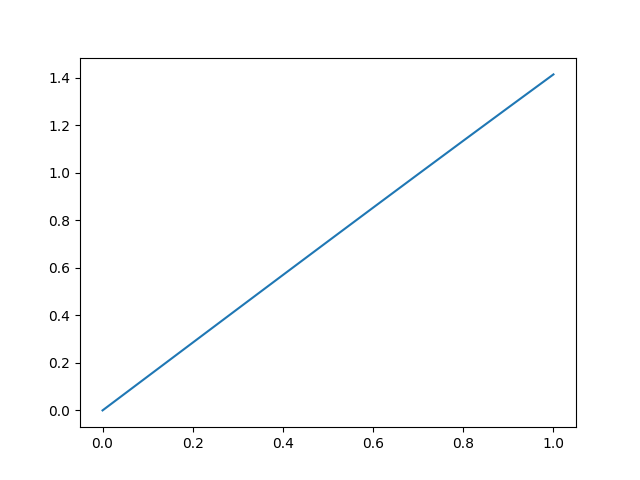
\includegraphics[width = 0.6\linewidth]{plot.png}
		\end{figure}
		\begin{figure}[h]
			\centering
			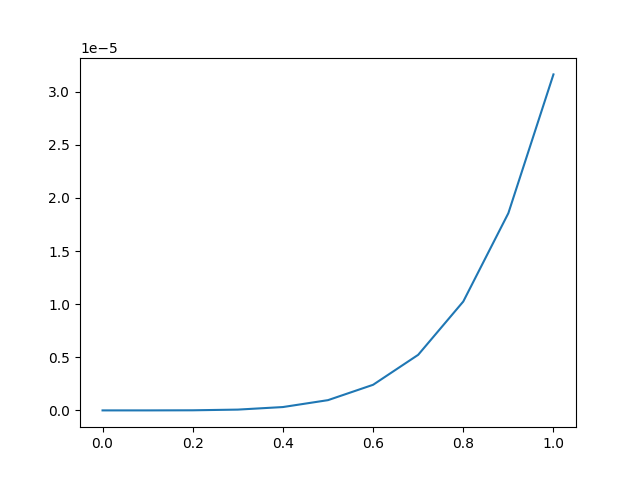
\includegraphics[width = 0.6\linewidth]{plot2.png}
			\caption{График погрешности}
		\end{figure}
		
		\pagebreak
		\pagebreak
		\subsection{Код программы}
			\lstinputlisting[language=Python]{./lab_5.py}
\end{document}	